\documentclass{beamer}
\usepackage{ctex, hyperref}
\usepackage[T1]{fontenc}

% other packages
\usepackage{latexsym,amsmath,xcolor,multicol,booktabs,calligra}
\usepackage{graphicx,pstricks,listings,stackengine}

\author{MashPlant 李晨昊}
\title{TrivialCompiler技术报告}
\date{2020年12月22日}
\usepackage{Tsinghua}

% defs
\def\cmd#1{\texttt{\color{red}\footnotesize $\backslash$#1}}
\def\env#1{\texttt{\color{blue}\footnotesize #1}}
\definecolor{deepblue}{rgb}{0,0,0.5}
\definecolor{deepred}{rgb}{0.6,0,0}
\definecolor{deepgreen}{rgb}{0,0.5,0}
\definecolor{halfgray}{gray}{0.55}
\definecolor{BlackText}{RGB}{0, 0, 0}

\lstset{
    basicstyle=\ttfamily\small,
    keywordstyle=\bfseries\color{deepblue},
    emphstyle=\ttfamily\color{deepred},    % Custom highlighting style
    stringstyle=\color{deepgreen},
    rulesepcolor=\color{red!20!green!20!blue!20},
    frame=shadowbox,
}

\usepackage{caption}
\captionsetup{labelformat=empty}

\begin{document}

\kaishu
\begin{frame}
    \titlepage
    \begin{figure}[htpb]
        \begin{center}
            
\includegraphics[width=0.2\linewidth]{pic/Tsinghua_University_Logo.eps}
        \end{center}
    \end{figure}
\end{frame}

\begin{frame}
    \tableofcontents[sectionstyle=show,subsectionstyle=show/shaded/hide,subsubsectionstyle=show/shaded/hide]
\end{frame}


\section{简介}

\begin{frame}{简介}
    \begin{itemize}
        \item 2020 年全国大学生系统能力大赛编译系统设计赛参赛作品,排名第二,获得一等奖
        \item 我与陈晟祺,陈嘉杰组队完成
        \item 将类似C语言的源语言SysY语言编译到ARMv7-A,在树莓派上运行
    \end{itemize}
  \begin{figure}[htpb]
    \centering
    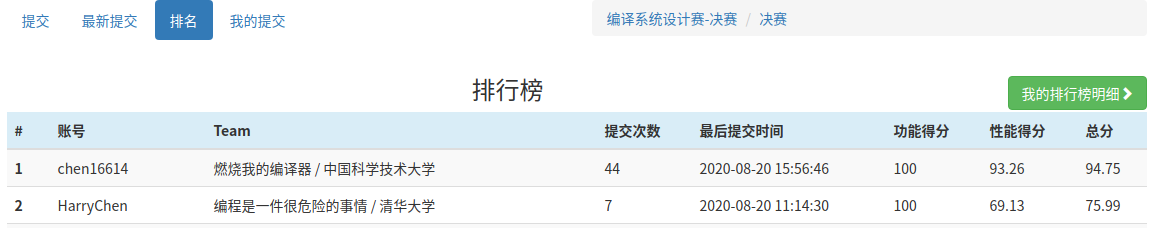
\includegraphics[width=1.0\linewidth]{pic/rank.png}
  \end{figure}
\end{frame}

\begin{frame}{架构}
\begin{itemize}
  \item C++17,基于CMake构建,代码量约6000行
  \item 从源文件经过 Lexing Parsing 构建 AST,类型检查,语义分析,然后转换成 SSA 形式的 IR,在IR上进行一系列的优化,再转化为机器码
  \item 我主要负责前端和IR上的优化,另外两人主要负责后端机器码生成
\end{itemize}
  \begin{figure}[htpb]
  \centering
  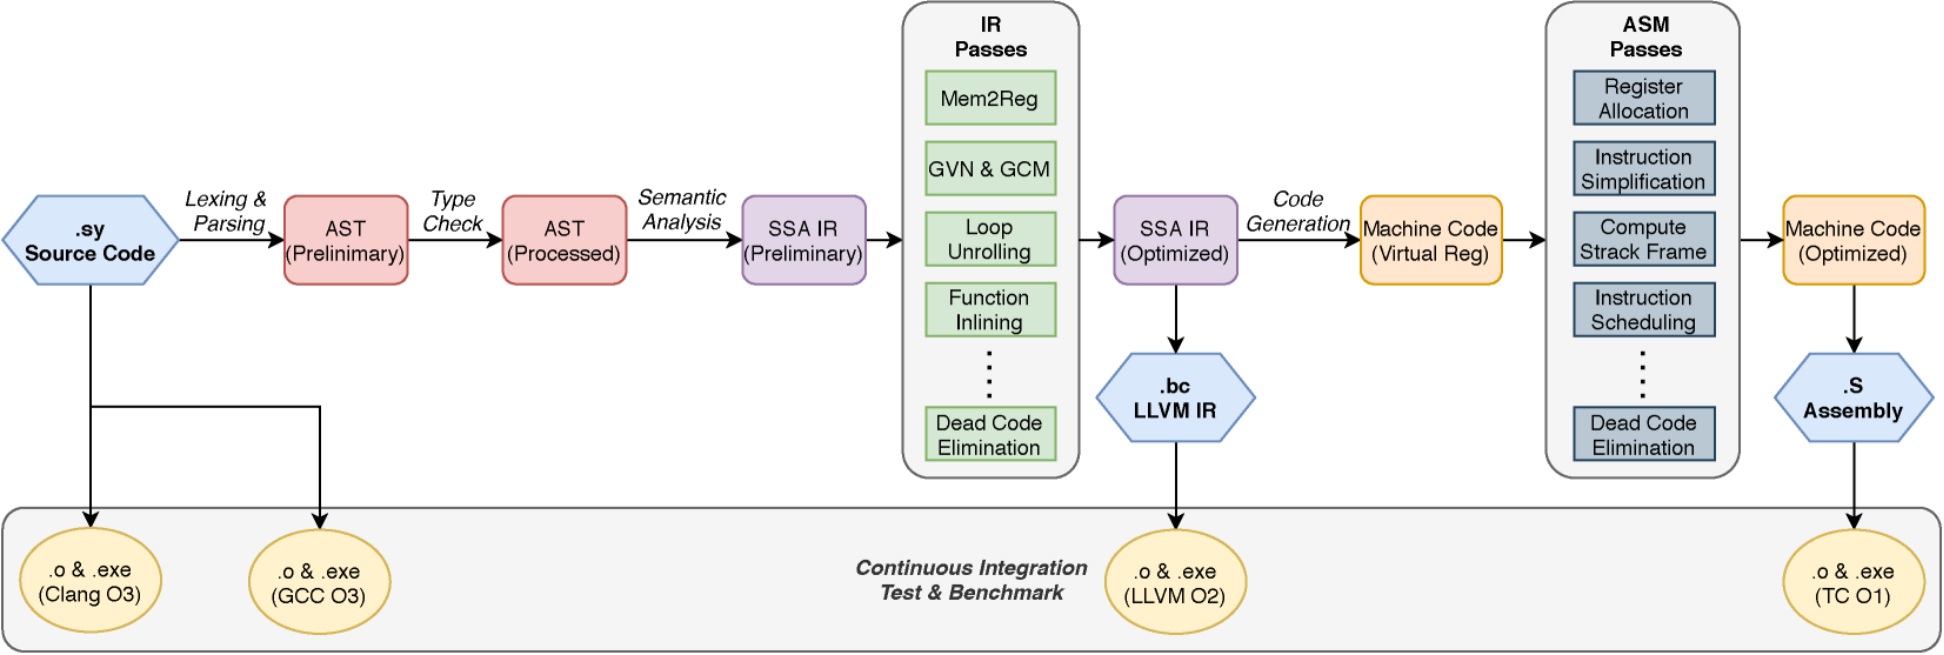
\includegraphics[width=1.0\linewidth]{pic/arch.png}
\end{figure}
\end{frame}

\section{前端}

\begin{frame}{前端}
\begin{itemize}
  \item Parser采用我编写的Parser Generator lalr1 \footnote{\href{https://github.com/MashPlant/lalr1}{https://github.com/MashPlant/lalr1}}自动生成
  \item lalr1内部调用re2dfa\footnote{\href{https://github.com/MashPlant/re2dfa}{https://github.com/MashPlant/re2dfa}}生成lexer
  \item lalr1采用龙书\footnote{Alfred V. Aho, Monica S. Lam, Ravi Sethi, and Jeffrey D. Ullman. 2006. Compilers: Principles, Techniques, and Tools (2nd Edition). Addison-Wesley Longman Publishing Co., Inc., USA.}中算法4.63描述的基于LR(0) FSM生成LALR(1)解析表的高效算法,在代码生成速度和生成的代码的执行速度上都超过了Yacc/Bison\footnote{基于C99文法(\href{http://www.quut.com/c/ANSI-C-grammar-y-1999.html}{http://www.quut.com/c/ANSI-C-grammar-y-1999.html})测试,测试输入选自\href{https://github.com/c-testsuite/c-testsuite}{https://github.com/c-testsuite/c-testsuite}}
\end{itemize}
\end{frame}

\begin{frame}{前端}
\begin{itemize}
  \item 今年的Rust版编译实验也采用lalr1,多数其他同学使用基于LL(*)文法的ANTLR
  \item ANTLR提供了更丰富的功能以简化文法的编写,但本质上都是编写产生式和语法动作
  \item ANTLR生成的代码需要配合Runtime使用,LL(*)文法的解析速度也较低;lalr1/Yacc/Bison都生成无依赖的代码
\end{itemize}
\end{frame}

\begin{frame}{编程技巧\footnote[1]{\href{https://llvm.org/docs/HowToSetUpLLVMStyleRTTI.html}{https://llvm.org/docs/HowToSetUpLLVMStyleRTTI.html}}}
\begin{itemize}
  \item AST节点和IR节点都涉及大量多态。C\texttt{++}原生的面向对象机制性能开销较大,在对象中保存一个整数值编码以判断实际类型,逻辑上与 \lstinline|dynamic_cast| 一样
  \item 访问节点的时候依据类型分别处理。这就是OOP引入Visitor模式时的反面写法,但我认为这样逻辑清晰,易于组合。这种写法与Visitor模式也不冲突,各有适用之处
\end{itemize}
\begin{figure}[htpb]
  \centering
  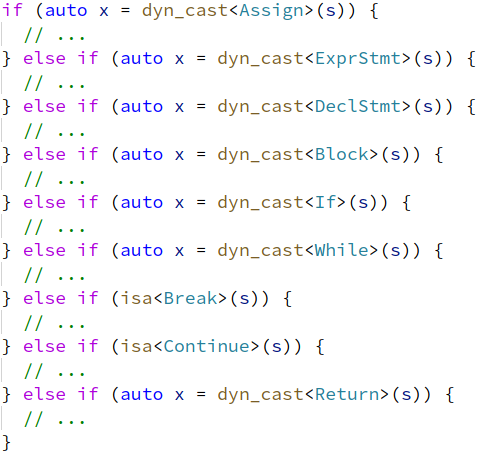
\includegraphics[width=0.35\linewidth]{pic/match.png}
\end{figure}
\end{frame}

\section{IR设计}

\begin{frame}{各种IR}
\begin{itemize}
  \item IR(Intermediate Representation):介于AST和机器码之间的一层,便于进行优化,分析,解释执行等工作
  \item IR有很多形式:基于栈的IR(Stack IR),基于虚拟寄存器的IR(Reg IR),SSA(Static Single Assignment) IR
  \begin{itemize}
    \item Stack IR:运算指令没有运算数,而是取出栈顶元素进行运算,将结果放回栈顶
    \item Reg IR:类似(RISC)汇编,有明确的操作数寄存器和目标寄存器,寄存器没有数量限制,一般一个变量对应一个寄存器
    \item SSA IR:类似Reg IR,但一个寄存器只能有一个赋值点,借助$\phi$函数实现多次对一个变量赋值的语义
  \end{itemize}
\end{itemize}
\end{frame}

\begin{frame}[fragile]{各种IR}

\begin{minipage}{1.0\linewidth}
\begin{lstlisting}[language=C]
int s = 0;
for (int i = 0; i < 100; i = i + 1) s = s + i;
\end{lstlisting}
\end{minipage}

\begin{minipage}{0.22\textwidth}
\begin{lstlisting}[caption = {Reg IR}, basicstyle = \fontsize{6}{6}\ttfamily\color{BlackText}]
  s = 0
  i = 0
L0:
  cond = i < 100
  br cond, L1, L2
L1:
  s = s + i
  i = i + 1
  br L0
L2:
\end{lstlisting}
\end{minipage}\hspace{1cm}
\begin{minipage}{0.36\textwidth}
\begin{lstlisting}[caption = {SSA IR}, basicstyle = \fontsize{6}{6}\ttfamily\color{BlackText}, escapeinside={(*@}{@*)}]
L0: 
  br L1
L1:
  s0 = (*@$\phi$@*) [0, L0], [s1, L2]
  i0 = (*@$\phi$@*) [0, L0], [i1, L2]
  cond = i0 < 100
  br cond, L2, L3
L2:
  s1 = s0 + i0
  i1 = i0 + 1
  br L1
L3:
\end{lstlisting}
\end{minipage}\hspace{1cm}
\begin{minipage}{0.16\textwidth}
\begin{lstlisting}[caption = {Stack IR}, basicstyle = \fontsize{6}{6}\ttfamily\color{BlackText}]
  const 0
  store s
  const 0
  store i
L0:
  load i
  const 100
  binary_lt
  br L1, L2
L1:
  load s
  load i
  binary_add
  store s
  load i
  const 1
  binary_add
  store i
  br L0
L2:
\end{lstlisting}
\end{minipage}
\end{frame}

\begin{frame}{各种IR}
\begin{table}[]
  \centering
  \begin{tabular}{|c|c|c|c|}
    \hline
    & Stack IR & Reg IR & SSA IR \\ \hline
    优化 & \textcolor[rgb]{1,0,0}{困难}       & 中等     & \textcolor[rgb]{0,1,0.2}{容易}     \\ \hline
    生成 & \textcolor[rgb]{0,1,0.2}{容易}       & 中等     & \textcolor[rgb]{1,0,0}{困难}     \\ \hline
    传输 & \textcolor[rgb]{0,1,0.2}{容易}\footnote[1]{虽然Stack IR的指令条数多,但指令中不用编码操作数,每条指令所占空间少}       & 中等     & 中等     \\ \hline
    阅读 & \textcolor[rgb]{1,0,0}{困难}       & 中等     & \textcolor[rgb]{1,0,0}{困难}     \\ \hline
  \end{tabular}
\end{table}
\begin{itemize}
  \item 因为各自的特点,不同的IR有不同的使用场景
  \begin{itemize}
    \item Stack IR多用于网络传输,如JVM Bytecode,WebAssembly
    \item Reg IR多用于高层分析验证,如Rust MIR,和教学级编译器
    \item SSA IR多用于工业级编译器,如GCC,LLVM
  \end{itemize}
  \item TrivialCompiler使用SSA IR
\end{itemize}
\end{frame}

\begin{frame}[fragile]{SSA IR}
\begin{itemize}
  \item $\phi$函数必须位于基本块的开头
  \item $\phi\ [v_1, L_1] \ldots [v_n, L_n]$中,$L_1, \ldots, Ln$必须恰好是本基本块的所有前驱基本块(因而实现时无需在$\phi$函数中保存基本块)
  \item 若运行时从$L_i$基本块进入本基本块,则$\phi$函数的值是$v_i$
  \item {\bf 一个基本块开头所有$\phi$函数同时计算}
  \begin{itemize}
    \item 例如某基本块开头$a = \phi\ [b, L_1];\ b = \phi\ [a, L_1]$,语义是交换$a$和$b$的值,而不是都赋成$b$
  \end{itemize}
\end{itemize}
\begin{center}
\begin{minipage}{0.36\textwidth}
\begin{lstlisting}[basicstyle = \fontsize{6}{6}\ttfamily\color{BlackText}, escapeinside={(*@}{@*)}]
L0: 
  br L1
L1:
  s0 = (*@$\phi$@*) [0, L0], [s1, L2]
  i0 = (*@$\phi$@*) [0, L0], [i1, L2]
  cond = i0 < 100
  br cond, L2, L3
L2:
  s1 = s0 + i0
  i1 = i0 + 1
  br L1
L3:
\end{lstlisting}
\end{minipage}
\end{center}
\end{frame}

\begin{frame}{SSA IR}
\begin{itemize}
  \item 理论上可以用和Reg IR一样的数据结构表示,只是加上$\phi$函数,但这样无法利用一个寄存器只有一个赋值点的性质。怎样快速知道一个寄存器在哪里定义,被谁使用了
  \begin{itemize}
    \item 可以用整数表示寄存器,再维护一个数组记录每个寄存器的定义位置和使用位置
    \item LLVM使用更高效且更复杂的表示方法,感兴趣的同学可以参考\href{https://www.zhihu.com/question/41999500}{https://www.zhihu.com/question/41999500}
    \item TrivialCompiler中使用类似LLVM早期版本的表示方法
  \end{itemize}
\end{itemize}
\end{frame}

\section{IR上的优化}

\begin{frame}[fragile]{Mem2Reg}
\begin{itemize}
  \item 存在从AST直接生成SSA IR的方法,但我没有研究过,常规方法是生成``伪''SSA,再用Mem2Reg转化成真正的SSA
  \item SSA要求一个寄存器只能有一个赋值点,但可以向一片内存写入任意多次,``伪''SSA中把变量都对应到栈上的内存
  \item Mem2Reg将这样的内存访问转化为寄存器访问,它是之后一切基于SSA IR的优化的基础
\end{itemize}
\begin{center}
\begin{minipage}{0.28\textwidth}
  \begin{lstlisting}[basicstyle = \fontsize{6}{6}\ttfamily\color{BlackText}, escapeinside={(*@}{@*)}]
L0:
  s = alloca int
  i = alloca int
  br L1
L1:
  tmp0 = *i
  cond = tmp0 < 100
  br cond, L2, L3
L2:
  tmp1 = *s
  tmp2 = *i
  *s = tmp1 + tmp2
  tmp3 = *i
  *i = tmp3 + 1
  br L1
L3:
  \end{lstlisting}
\end{minipage}\hspace{0.5cm}
$\Rightarrow$
\hspace{0.4cm}
\begin{minipage}{0.35\textwidth}
  \begin{lstlisting}[basicstyle = \fontsize{6}{6}\ttfamily\color{BlackText}, escapeinside={(*@}{@*)}]
L0:
  br L1
L1:
  s0 = (*@$\phi$@*) [0, L0], [s1, L2]
  i0 = (*@$\phi$@*) [0, L0], [i1, L2]
  cond = i0 < 100
  br cond, L2, L3
L2:
  s1 = s0 + i0
  i1 = i0 + 1
  br L1
L3:
  \end{lstlisting}
\end{minipage}
\end{center}
\end{frame}

\begin{frame}{Mem2Reg}
\begin{itemize}
  \item 定义基本块的支配边界DF(Dominance Frontier):$DF(n) = \{ x | n\text{支配}x\text{的某个前驱,且}(n = x\text{或}n\text{不支配}x) \}$
  \item 集合的支配边界:$DF(S) = \bigcup_{n \in S} DF(n)$
  \item 集合的迭代支配边界:$DF_1(S) = DF(S);\ DF_{i + 1}(S) = DF(S \cup DF_i(S))$,迭代至收敛得到$DF^+(S)$
  \item 支配边界的高效计算用到后面提到的支配树,这里略过
\end{itemize}
\end{frame}

\begin{frame}{Mem2Reg}
\begin{itemize}
  \item 一个支配边界的例子\footnote[1]{\href{https://www.cs.colostate.edu/~mstrout/CS553Fall06/slides/lecture17-SSA.pdf}{https://www.cs.colostate.edu/\textasciitilde mstrout/CS553Fall06/slides/lecture17-SSA.pdf}}:
\end{itemize}
\begin{figure}[htpb]
  \centering
  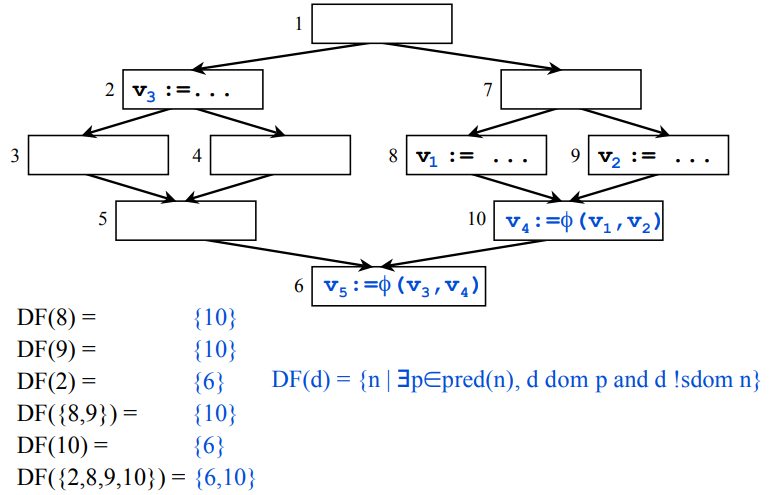
\includegraphics[width=0.8\linewidth]{pic/df.png}
\end{figure}
\end{frame}

\begin{frame}{Mem2Reg}
\begin{itemize}
  \item 第一步:收集对一个变量的所有写入的基本块集合$S$,为$DF^+(S)$中的每个基本块插入$\phi$函数
  \item 直观理解:在支配边界上这个变量从不同前驱来值可能不同,所以需要插入$\phi$函数。因为$\phi$函数本身也是一次定值,需要把插入的地方也考虑进去再计算$DF$,这就是$DF^+$的意义
  \item 实现时只计算每个基本块的$DF$,不计算$DF^+$,迭代插入$\phi$函数即可
\end{itemize}
\end{frame}

\begin{frame}{Mem2Reg}
\begin{itemize}
  \item 第二步:确定$\phi$的参数和load的结果。从起始节点开始DFS:
  \begin{itemize}
    \item 跳过基本块开头的$\phi$函数,对之后的每条语句:
    \begin{itemize}
      \item 对变量的store:删除它,记录变量最新的值是被store的值
      \item 对变量的load:删除它,对它的使用替换成变量最新的值
    \end{itemize}
    \item 访问完语句后,依次访问基本块的所有后继。对一个后继先访问它开头的$\phi$函数,将属于这个变量的$\phi$对应位置替换成变量最新的值,然后记录变量最新的值是这个$\phi$,然后访问这个基本块
    \item 全部后继访问完后,恢复进入这个基本块时变量的值(可以用栈实现)
  \end{itemize}
\end{itemize}
\end{frame}

\begin{frame}{GVN \& GCM \footnote[1]{Cliff Click. 1995. Global code motion/global value numbering. SIGPLAN Not. 30, 6 (June 1995), 246–257.}}
\begin{itemize}
  \item GVN \& GCM可以消除冗余计算,提取循环不变式,减轻寄存器压力,代数简化,常量折叠\ldots
  \item GVN:按照某个顺序访问所有表达式,如果$e_2$和之前遇到的$e_1$运算类型相同且参数的value numbering相同,那么$e_2$和的$e_1$的value number相同,可以用$e_1$替换$e_2$
  \begin{itemize}
    \item 内存访问也可以处理,将内存操作依赖的内存操作视作参数,LLVM中有MemorySSA模块,TrivialCompiler也初步实现了
    \item 在这一步顺便进行代数简化,常量折叠
  \end{itemize}
  \item 这样生成的程序可能是不合法的,一个表达式不一定在使用它前被计算,通过GCM使之合法
\end{itemize}
\end{frame}

\begin{frame}{GVN \& GCM}
\begin{itemize}
  \item 定义基本块直接支配关系$x\ idom\ y$:$x$支配$y$,且不支配任何支配$y$的其他节点
  \item 除开始节点外每个节点恰被一个节点直接支配,这构成一棵树,称作支配树
  \item 节点在支配树中的深度称作支配深度。直观理解支配深度更大,就被更多层if语句包裹,更有可能不执行
\end{itemize}
\hspace{1cm}
\begin{minipage}{0.3\linewidth}
\begin{figure}[htpb]
  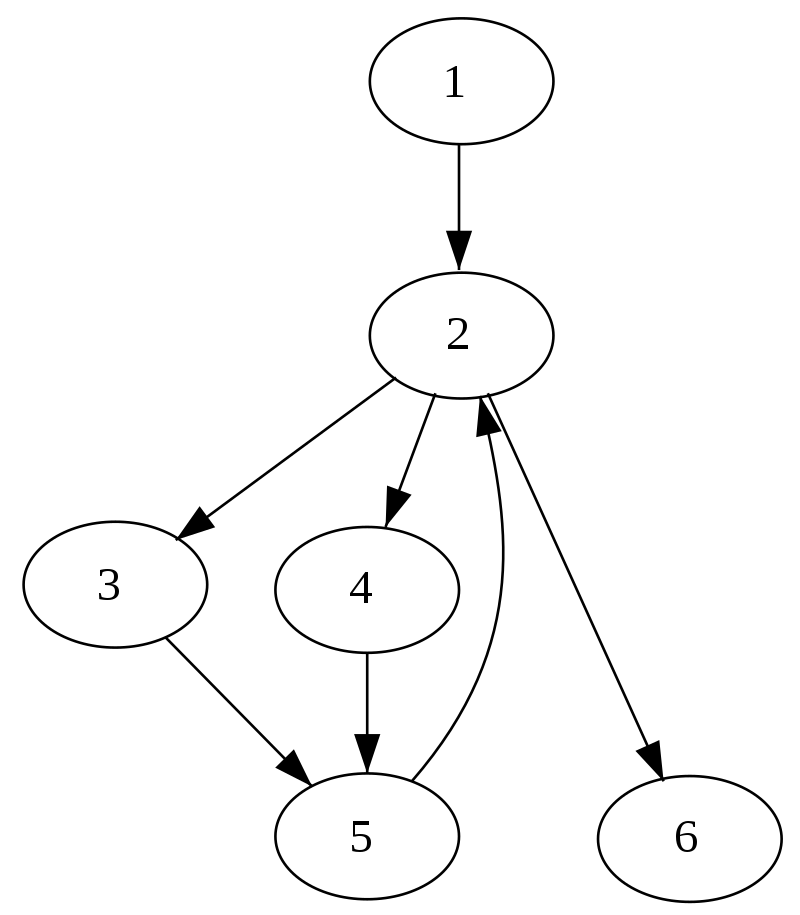
\includegraphics[width=1.0\linewidth]{pic/cfg.png}
\end{figure}
\end{minipage}\hspace{1cm}
\begin{minipage}{0.37\linewidth}
  \begin{figure}[htpb]
    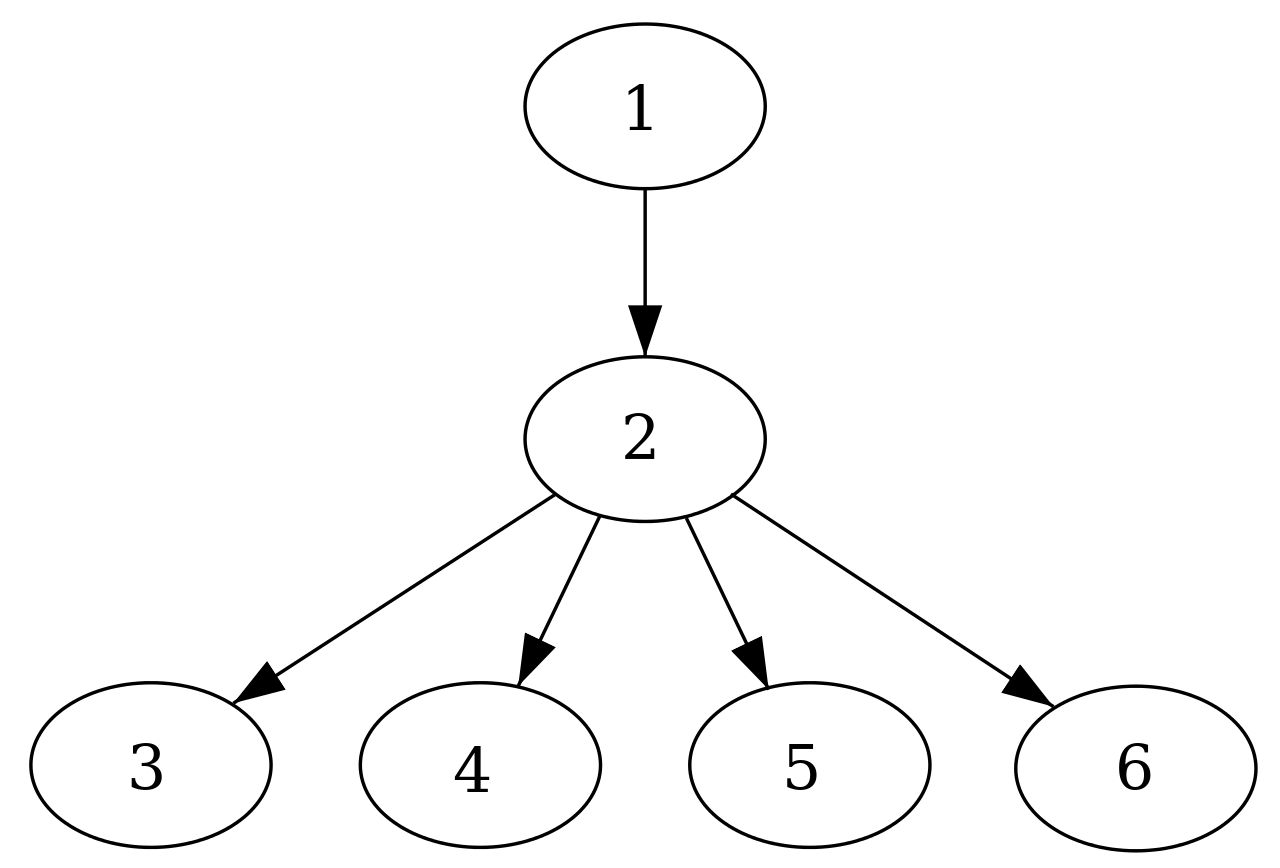
\includegraphics[width=1.0\linewidth]{pic/dom_tree.png}
  \end{figure}
\end{minipage}
\end{frame}

\begin{frame}{GVN \& GCM}
\begin{itemize}
\item GCM:先移动到到尽量早的位置,再移动到到尽量晚的位置
\item \lstinline|schedule_early| :依次用 \lstinline|schedule_early| 调度所有参数,如果一个参数所在基本块支配深度小于自身,就将自身移动到参数的基本块。这样可以保证自身被参数支配
\item \lstinline|schedule_late| :先用 \lstinline|schedule_late| 调度所有使用者,从支配树上所有使用者的LCA到原始位置的一条链上都是可行的位置,选择循环嵌套层次最浅,支配深度尽量深的
\item GCM不关心基本块内指令的顺序,有专门的局部调度算法
\end{itemize}

\end{frame}
\section{机器码生成及优化}

\begin{frame}{指令选择}
\begin{itemize}
  \item 通常编译器后端先进行指令选择,再进行优化和寄存器分配
  \item 指令选择将IR指令翻译到带有虚拟寄存器和机器寄存器的机器指令,机器寄存器用于满足调用约定等需求
  \item SSA IR中运算,访存,函数调用等指令的翻译与Reg IR类似,但指令集中一般没有$\phi$函数,需要翻译成赋值语句
  \begin{itemize}
    \item 对于$x = \phi\ [v_1, L_1] \ldots [v_n, L_n]$,在$L_i$末尾生成$x = v_i$
    \item 如果有多个$\phi$函数$\phi_1, ..., \phi_m$,赋值$x_1 = v_{i1}; \ldots; x_m = v_{im}$必须是并行执行的,一种实现方式是先把$v_{i1}, \ldots, v_{im}$赋给$t_1, \ldots, t_m$,再把$t_1, \ldots, t_m$赋给$x_1, \ldots, x_m$
  \end{itemize}
\end{itemize}
\end{frame}

\begin{frame}{窥孔优化}
\begin{itemize}
  \item TrivialCompiler中利用ARMv7-A指令集进行了很多窥孔优化,这里介绍除常数优化
  \item 很多处理器上除法都是非常耗时的操作,除法的延迟可达加法的几十倍,而乘法的延迟和加法在一个数量级。除常数是一种常见的操作,希望能够避免用除法计算它
  \item \lstinline|int i|,\lstinline|i / 2| 可以优化成 \lstinline|i >> 1| 吗?
  \pause
  \item 不能!整数除法向0取整,\lstinline|-1 / 2 == 0|,\lstinline|-1 sra 1 == -1|
  \item \lstinline|i / 2021|又该怎么优化呢?
\end{itemize}
\end{frame}

\begin{frame}{窥孔优化}
\begin{itemize}
  \item TrivialCompiler采用论文中\footnote[1]{Torbjörn Granlund and Peter L. Montgomery. 1994. Division by invariant integers using multiplication. SIGPLAN Not. 29, 6 (June 1994), 61–72. DOI:https://doi.org/10.1145/773473.178249}描述的除常数优化算法
  \item \lstinline|i / 2 == (i + (i < 0)) >> 1|
  \item \lstinline|i / 2021 == ((i + ((int64(-2118793861) * i) >> 32))| \lstinline|>> 10) + (i < 0)|
  \pause
  \item 很多人习惯使用带符号整数,但一些场景下这限制了编译器的优化,无符号整数除常数生成的代码更精简
\end{itemize}
\end{frame}

\begin{frame}{寄存器分配}
\begin{itemize}
  \item TrivialCompiler采用论文\footnote[1]{Lal George and Andrew W. Appel. 1996. Iterated register coalescing. ACM Trans. Program. Lang. Syst. 18, 3 (May 1996), 300–324. DOI:https://doi.org/10.1145/229542.229546}中描述的图着色寄存器分配算法
  \item 指令选择生成的代码中存在大量赋值语句,通过寄存器分配解决这个问题:如果赋值左右操作数被分配到同一个寄存器,这次赋值就可以去掉
  \item 论文中有更详细的描述和伪代码,这里只大致介绍重要思想
\end{itemize}
\end{frame}

\begin{frame}{寄存器分配}
\begin{minipage}{0.75\linewidth}
  \begin{itemize}
    \item 构建干涉图:与课中描述的类似,但特殊处理赋值:即使右操作数在赋值语句后存活,也不用在左右操作数间连边
    \item 对机器寄存器预着色,预着色的节点间互相不同色,着色过程中也不再分配颜色
    \item 着色过程:选择度数小于机器寄存器数目的节点删除之,若不存在则按照启发式算法选择一个。同时尝试进行节点合并,freeze等操作。重复直至删除完,逆序添加回去,为每个节点选择邻居都没有的颜色,若没有可用的颜色证明它需要spill,分配完成后依据需要spill的节点重写程序,再分配一次
  \end{itemize}
\end{minipage}
\begin{minipage}{0.2\linewidth}
  \begin{figure}[htpb]
    \centering
    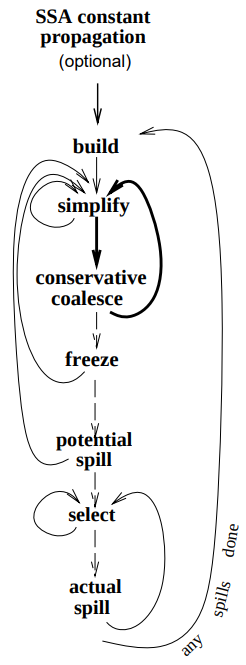
\includegraphics[width=1.0\linewidth]{pic/reg.png}
  \end{figure}
\end{minipage}
\end{frame}

\begin{frame}
    \begin{center}
        {\Huge\calligra Thanks!}
    \end{center}
\end{frame}

\end{document}